\section{M\'etodo de im\'agenes, funci\'on de Green y separaci\'on de variables}

\subsection{}
En este problema, tenemos una esfera conductora de radio $a$ conectada a un potencial $V$, rodeada por otra c\'ascara esf\'erica de radio $b$ con densidad superficial de carga $\sigma$

\begin{figure}[H]
  \centering
  \begin{subfigure}[b]{0.7\linewidth}
    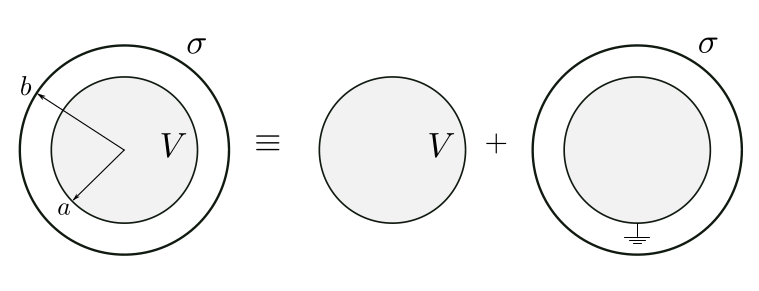
\includegraphics[width=\linewidth]{Guia2/g2_e1_im.png}
  \end{subfigure}
  \caption{Diagrama de la configuraci\'on dada.}
  \label{fig:g2_e1_im}
\end{figure}

\begin{itemize}
    \item En el punto a) queremos hallar $\Phi$ en todo el espacio usando el m\'etodo de im\'agenes con la superposici\'on propuesta en la figura (\ref{fig:g2_e1_im}). Esto nos permite escribir el potencial como la siguiente suma:

    $$\Phi(\mathbf{r}) = \Phi_{CC}(\mathbf{r}) + \Phi_{\sigma}(\mathbf{r})$$

    donde $\Phi_{CC}(\mathbf{r})$ es el potencial de la esfera a $V$ y $\Phi_{\sigma}(\mathbf{r})$ el del cascar\'on con densidad $\sigma$ y la esfera a tierra.

    El potencial $\Phi_{CC}$ decae como $\frac{1}{r}$ fuera de la esfera, y es igual a $V$ dentro de ella, luego por continuidad debe ser $\frac{Va}{r}$. Si utilizamos la notaci\'on  
    
    $$r_{>~}^{(a)} = max[r, a]$$

    Dicho potencial nos quedar\'a finalmente

    $$\Phi_{CC}(\mathbf{r}) = \frac{Va}{r_{>~}^{(a)}}$$

    donde $Va$ es la carga inducida sobre la esfera a potencial $V$.\\
    
    Para el potencial de la c\'ascara y la esfera a tierra, $\Phi_{\sigma}$, podemos tomar a cada elemento infinitesimal de la c\'ascara como una carga puntual con una carga imagen asociada (dentro de la c\'ascara). Particularmente, como todos los puntos son equivalentes, cada imagen se encuentra a la misma distancia del origen, es decir

    $$r' = \frac{a^{2}}{b}$$

    Por \'ultimo, para $r \geq a$, el potencial de la c\'ascara frente a la esfera es el potencial de dos c\'ascaras: una de radio $b$ y carga $Q$ y su imagen de radio $r'$ y carga $Q' = -\frac{a}{b}Q$:

    \[\Phi_{\sigma}(\mathbf{r})=
        \begin{cases}
            \frac{Q'}{r_{>~}^{(r')}} + \frac{Q}{r_{>~}^{(b)}} = Q\bigg(-\frac{a}{br} + \frac{1}{r_{>~}^{(b)}}\bigg) & r \geq a\\
            0  & r \leq a
        \end{cases}
    \]

    donde $r_{>~}^{(r')} = r$ en la regi\'on $r \geq a$. Luego, el potencial total del problema ser\'a

    \[\Phi(\mathbf{r}) = \Phi_{CC}(\mathbf{r}) + \Phi_{\sigma}(\mathbf{r})
        \begin{cases}
            \frac{Va}{r} Q\bigg(-\frac{a}{br} + \frac{1}{r_{>~}^{(b)}}\bigg) & r \geq a\\
            V & r \leq a
        \end{cases}
    \]

    \item La carga total inducida sobre la esfera ser\'a

    $$Q_{TOT} = Va + Q'$$
\end{itemize}

\subsection{}
Veamos el problema anterior pero utilizando la funci\'on de Green. La mayoría de las veces vamos a utilizar las condiciones de contorno de Dirichlet, entonces podemos escribir el potencial electrost\'atico de la siguiente manera

\begin{equation}
    \label{eq:green_dirichlet}
    \Phi(\mathbf{r}) = \int_{V}d^{3}\mathbf{r}'\rho(\mathbf{r}')G(\mathbf{r}, \mathbf{r}') - \frac{1}{4\pi}\oint_{S}d^{2}r'\frac{\partial G(\mathbf{r}, \mathbf{r}')}{\partial n'}\Phi(\mathbf{r}')
\end{equation}

donde el valor del potencial en $S$ es dato.\newline

Como en el problema, si las cargas en volumen est\'an distribuidas sobre una superficie $\Sigma$, el primer t\'ermino de (\ref{eq:green_dirichlet}) es una integral de superficie

$$\int_{V}d^{3}\mathbf{r}'\rho(\mathbf{r}')G(\mathbf{r}, \mathbf{r}') = \int_{\Sigma}d^{2}r'\sigma(\mathbf{r}')G(\mathbf{r}, \mathbf{r}')$$

En nuestro caso, las integrales que est\'an sobre las superficies de radio $a$ (contorno) y $b$ (cargas), quedan

$$\int_{\Sigma}d^{2}r' \rightarrow \int_{r' = a, b}d^{2}r'$$

Adem\'as, como el volumen del problema es en la regi\'on $r > a$, la normal exterior es $\mathbf{n}' = -\hat{r}'$, luego $\frac{\partial}{\partial n'} = -\frac{\partial}{\partial r'}$. Con toda esta informaci\'on, la ecuaci\'on (\ref{eq:green_dirichlet}) nos queda

\begin{equation}
    \label{eq:green1}
    \Phi(\mathbf{r}) = \int_{r' = b}d^{2}r'G(\mathbf{r}, \mathbf{r}')\sigma + \frac{V}{4\pi}\int_{r' = a}d^{2}r'\frac{\partial G(\mathbf{r}, \mathbf{r}')}{\partial r'}
\end{equation}

Luego, la funci\'on de Green correspondiente es

\begin{equation}
    \label{eq:green2}
    G(\mathbf{r}, \mathbf{r}') = \frac{1}{|\mathbf{r} - \mathbf{r}'|} - \frac{a}{r'}\frac{1}{|\mathbf{r} - \frac{a^{2}}{r'^{2}}\mathbf{r}'|}
\end{equation}

En este punto, hay varios m\'etodos para resolver la ecuaci\'on (\ref{eq:green1}), vamos a utilizar la expansi\'on en arm\'onicos esf\'ericos de la funci\'on de Green. La primer integral de dicha ecuaci\'on puede escribirse en funci\'on del \'angulo s\'olido de la siguiente manera

$$ \Phi_{V}(\mathbf{r}) = \int_{r' = b}d^{2}r'G(\mathbf{r}, \mathbf{r}')\sigma = \int_{r' = b}b^{2}d\Omega G(\mathbf{r}, \mathbf{r}')\sigma$$

donde la integral angular es sobre el vector $\mathbf{r}'$

$$\int d\Omega \rightarrow \int_{0}^{2\pi} d\phi' \int_{-1}^{1}\sin \theta' d\theta'$$

La funci\'on de Green expresada en arm\'onicos esf\'ericos es

\begin{equation}
    \label{eq:green3}
    G(\mathbf{r}, \mathbf{r}') = \sum_{lm} \frac{4\pi}{2l + 1}Y_{lm}(\theta, \phi)Y_{lm}^{*}(\theta', \phi')\bigg[ \frac{r^{l}_{<~}}{r^{l+1}_{>~}} - \frac{a^{2l + 1}}{(rr')^{l+1}}\bigg]
\end{equation}

$$\Rightarrow \Phi_{V}(\mathbf{r}) = \sum_{lm} \frac{4\pi \sigma}{2l + 1}\bigg[ \frac{r^{l}_{<~}}{r^{l+1}_{>~}} - \frac{a^{2l + 1}}{(rr')^{l+1}}\bigg]_{r' = b}\bigg[Y_{lm}(\theta, \phi)\int b^{2}d\Omega Y_{lm}^{*}(\theta', \phi')\bigg]$$

Un buen truco es escribir la integral de $Y_{lm}^{*}(\theta', \phi')$ como el producto escalar con $1 = \sqrt{4\pi}Y_{00}(\theta', \phi')$, entonces $\int b^{2}d\Omega Y_{lm}^{*}(\theta', \phi') = \sqrt{4\pi}\int b^{2}d\Omega Y_{lm}^{*}(\theta', \phi')Y_{00}(\theta', \phi') = \sqrt{4\pi}\delta_{l, 0}\delta_{m, 0}$.\\

Luego en $\Phi_{V}(\mathbf{r})$ quedan solo los t\'erminos con $m = l = 0$, entonces

$$\Phi_{V}(\mathbf{r}) = 4\pi b ^{2}\sigma\bigg[ \frac{1}{r_{>~}} - \frac{a}{br}\bigg] = Q\bigg[ \frac{1}{r_{>~}} - \frac{a}{br}\bigg]$$\\

La contribuci\'on del potencial en la superficie es

$$ \Phi_{S}(\mathbf{r}) = \frac{V}{4\pi}\int_{r' = a}d^{2}r'\frac{\partial G(\mathbf{r}, \mathbf{r}')}{\partial r'}$$\\

Ac\'a tenemos que $r_{<~} = r'$ y $r_{>~} = r$, por lo tanto

$$\Phi_{S}(\mathbf{r}) = \frac{V}{4\pi} \sum_{lm} \frac{4\pi}{2l + 1}(2l + 1) \frac{a^{l - 1}}{r^{l+1}}\bigg[ Y_{lm}(\theta, \phi)\int a^{2} d\Omega Y_{lm}^{*}(\theta', \phi')\bigg] = \frac{Va}{r}$$

\subsection{}
En la siguiente im\'agen vemos un esquema del problema

\begin{figure}[H]
  \centering
  \begin{subfigure}[b]{0.3\linewidth}
    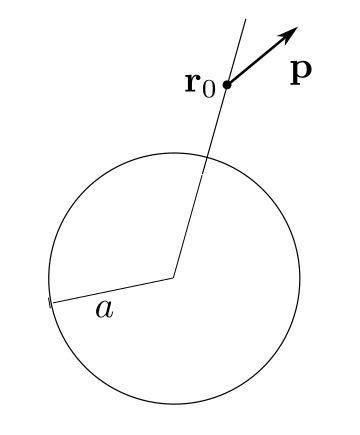
\includegraphics[width=\linewidth]{Guia2/g2_dipolo.png}
  \end{subfigure}
  \caption{Diagrama de la configuraci\'on.}
  \label{fig:g2_dipolo}
\end{figure}


donde $\mathbf{p}$ es un dipolo ubicado en el punto $\mathbf{r}_{0}$ junto a una esfera de radio $a$. Tenemos que calcular el potencial en todo el punto del espacio

\begin{itemize}
    \item M\'etodo de la funci\'on de Green

    \item M\'etodo de im\'agenes
\end{itemize}